\documentclass[10pt,a4paper,titlepage]{article}
\usepackage[utf8]{inputenc}
\usepackage[frenchb]{babel}
\usepackage{fontenc}
\usepackage{amsmath}
\usepackage{amsfonts}
\usepackage{amssymb}
\usepackage{makeidx}
\usepackage{graphicx}
\author{Éric Quinton}
\title{Organiser les données en s'appuyant sur les traitements}
\begin{document}
Depuis quelques mois, je travaille dans un centre de recherche. Alors que les chercheurs manipulent des quantités souvent importantes de données, ils n'en maîtrisent que rarement la manière de les stocker ou d'y accéder. 
Il n'est pas rare de trouver des fichiers Excel de plusieurs milliers de lignes et de dizaines de colonnes, avec tout ce que cela entraîne : redondance des fichiers (un fichier par version), données mal formatées, et donc mal traitées ensuite, etc. Dans le meilleur des cas, ils ont recours à des fichiers Access, ce qui ne vaut guère mieux : le logiciel mélange allègrement les requêtes et les données, et s'y retrouver devient parfois compliqué.
Cela se traduit par des pertes de temps importantes au moment d'exploiter les informations, voire à une impossibilité d'être sûr que les résultats obtenus sont bien cohérents avec les données manipulées.

Tous les laboratoires ne peuvent pas investir dans des administrateurs de bases de données. Non seulement ces profils ne sont pas fréquents, mais avec la baisse des effectifs, recruter une telle personne ne peut se faire qu'au détriment d'autre chose. De plus, certains chercheurs rechignent à laisser leurs données entre les mains de personnes tierces, qui pourraient remettre en question leur approche initiale et la conception qu'ils avaient de la structuration des données.

Pour s'en sortir, les chercheurs essaient de se former comme ils le peuvent à la gestion des données. Certains séminaires sont même dédiés à ce sujet.

Cette approche me laisse aujourd'hui perplexe. Dès lors que les données sont vues comme une entité immuable, intrinsèque, la tendance est de figer leur structuration \og dans le marbre \fg . De fait, les chercheurs se tournent facilement vers d'anciennes méthodes comme Merise, qui sont centrées sur les données.
Des choix d'organisation sont alors érigés souvent en principes et appliqués à tout type de problème : des structures de type \og entités - relations \fg (je reviendrai sur ce type d'organisation), qui présentent des avantages dans certains cas, sont appliqués à des domaines desquelles elles devraient être exclues.

\section{Qu'est-ce qu'une donnée ?}
La première approche consiste à s'appuyer sur le dictionnaire pour en obtenir une définition. Voici un extrait de celle du dictionnaire Larousse \cite{donnee_larousse} :
\og 
\begin{itemize}

\item \og (...)
\item Représentation conventionnelle d'une information en vue de son traitement informatique.
\item Résultats d'observations ou d'expériences faites délibérément ou à l'occasion d'autres tâches et soumis aux méthodes statistiques.
\item (...)\fg

\end{itemize}

La notion de \textit{représentation} est probablement la plus importante. Une donnée n'est qu'un artefact d'un objet, qui permet de le représenter d'une manière conceptuelle, de telle façon que toute personne disposant du cadre de référence utilisé pour la générer puisse l'interpréter sensiblement de la même façon. 
Pour exprimer cela de manière plus claire, regardez ce tableau de Magritte :
\begin{center}
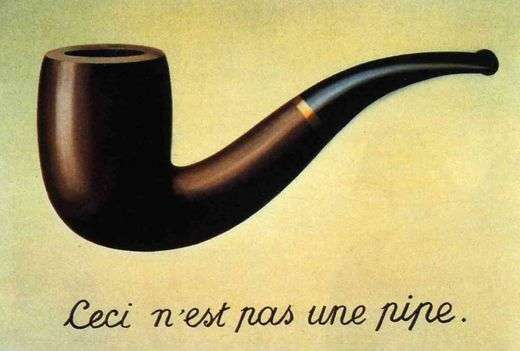
\includegraphics{image/pipe}
\end{center}
Il est sous-titré : \og Ceci n'est pas une pipe\fg. Le dessin, aussi suggestif et proche de la vision que toute personne peut avoir d'une pipe, n'en est qu'une représentation, qui plus est uniquement visuelle : pas question d'en approcher l'odeur, la texture, le poids ! Toutefois, implicitement, nous avons tendance à dire qu'il s'agit bien d'une pipe : nous \og sautons\fg l'étape intermédiaire de représentation pour traduire le dessin en concept, en considérant que l'information visuelle fournie est un objet réel.

Il en est de même pour les données : une fois exprimées, il est assez facile de considérer qu'elles peuvent se substituer à la réalité, et acquièrent, de ce fait, une existence par elles-mêmes. Ce serait, bien sûr, une erreur.

La principale conséquence de cette approche, c'est que la donnée n'a pas de valeur intrinsèque. Elle ne doit être abordée qu'en fonction de ce qu'on veut lui faire représenter, et elle n'est qu'un artefact de la réalité.
Ainsi, elle ne devrait pas être traitée ou manipulée en dehors de son contexte, que celui-ci soit clairement exprimé, ou implicite. 
Prenons un autre exemple : en citant cette assertion : \og la taille de cet objet est de 20 cm\fg. Nous en déduisons que la taille globale de l'objet s'insère dans un système de mesure dont l'étalon, le mètre, correspond à une unité référencée, et qu'elle a été mesurée avec un mécanisme permettant d'obtenir une précision de l'ordre du centimètre, voire plus faible. Le même objet, annoncé avec une dimension de 20,248 cm, exprime une donnée bien différente. La précision fournie indique que le procédé de mesure n'est pas identique : c'est bien le contexte implicite qui permet de caractériser l'information fournie.


\bibliographystyle{plain}
\bibliography{donnees_biblio}


\end{document}